\documentclass[8pt]{beamer}
\usepackage[nobglogo]{beamerthemedmi-owled}
\usepackage[utf8x]{inputenc}
\usepackage{default}
\usepackage{url}
\usepackage{verbatim}
\usepackage{graphicx}
\usepackage{mathrsfs}
\usepackage{dl}
\usepackage{mls}
%\usepackage{listings}


\mode<presentation>
{
  \usetheme{dmi-owled}
  %\usetheme{Warsaw}
  % or ...

  \setbeamercovered{transparent}
  % or whatever (possibly just delete it)
}

\title{Introduzione agli Open Data}

\author{Cristiano Longo\\ 
{\small{longo@dmi.unict.it}}}



\date{Universit\`a di Catania, 13 Maggio 2015}
\newcommand{\urlsingle}[1]{{\small {\center {\url{#1}}}}}
\begin{document}
\maketitle
\setcounter{tocdepth}{1}

\section{Introduzione}


\begin{frame}
\frametitle{Definizione}

\begin{quote}
Open means anyone can freely access, use, modify, and share for any purpose (subject, at most, to requirements that preserve provenance and openness).\footnote{\url{http://opendefinition.org}} 
\end{quote}

da \emph{Open Knowledge Foundation: The Open Definition}
\end{frame}

\begin{frame}
\frametitle{Cenni \emph{Storici}}

La \emph{Open Definition} deriva dalla \emph{Open Source Definition}\footnote{\url{http://www.opensource.org/docs/osd}},
che deriva a sua volta dalle \emph{Debian Free Software Guidelines}\footnote{\url{http://www.debian.org/social_contract}}.
\vspace{\baselineskip}

\uncover<1->{
In queste linee guida vengono riportati alcuni esempi di licenze \emph{libere}:
GPL,\footnote{\url{http://www.gnu.org/copyleft/gpl.html}}
BSD,\footnote{\url{http://www.debian.org/misc/bsd.license}}
Artistic.\footnote{\url{http://perldoc.perl.org/perlartistic.html}}
}
\vspace{\baselineskip}

\uncover<2->{
Le implicazioni e le potenzialit\`a della libera circolazione del pensiero
erano note gi\`a da tempo:
\vspace{\baselineskip}

\begin{quote}
Se io ho una mela, tu hai una mela e ce le scambiamo, abbiamo sempre una
mela per uno. Ma se io ho una idea e tu hai un'altra idea e ce le scambiamo,
avremo due idee ciascuno. 
\end{quote}
\emph{G.B. Shaw}
}
\end{frame}

\begin{frame}
\frametitle{Ricadute (1/1)}

Oggi le ricadute dell'apertura dei dati sono pi\`u chiare ed evidenti.
Ad esempio, parlando di \emph{Europeana}\footnote{\url{http://europeana.eu}},
Neelie Kroes, della Commissione Europea, dice:
\vspace{\baselineskip}

\begin{quote}
Europe has probably the world’s greatest cultural heritage. Digitisation brings
culture into people’s homes and is a valuable resource for education, tourism,
games, animation and the whole creative industry. Investing in digitisation will
create new companies and generate new jobs.
\end{quote}
\end{frame}

\begin{frame}
\frametitle{Ricadute dell'Apertura di Dati Pubblici}
Alcune ricadute dell'apertura dei dati, in particolare di quelli in possesso 
della Pubblica Amministrazione, possono essere classificati come segue:
\vspace{\baselineskip}

\begin{itemize} [<+->]
 \item economici
 \begin{itemize}
  \item redazione di business plan
  \item creazione di nuove imprese basate sui dati (vedi ad esempio \emph{Open Data 500}\footnote{\url{http://www.opendata500.com/us/list/}})
 \end{itemize}
 \item realizzazione di nuovi servizi per i cittadini (vedi ad esempio TODO \emph{Travic}\footnote{\url{tracker.geops.ch/}})
 \item trasparenza (vedi ad esempio \url{soldipubblici.it} oppure \url{http://parlamento17.openpolis.it/})
 \item governo partecipato (uno strumento ad esempio è \url{http://www.normattiva.it/}).
\end{itemize}
\end{frame}

\begin{frame}
\frametitle{Definizione}

\begin{quote}
Open means anyone can freely access, use, modify, and share for any purpose (subject, at most, to requirements that preserve provenance and openness).\footnote{\url{http://opendefinition.org}} 
\end{quote}
\vspace{\baselineskip}

Per rendere effettiva questa definizione \`e necessario prendere in considerazione
diversi aspetti.
\vspace{\baselineskip}

\begin{itemize}[<+->]
 \item \emph{Tecnici} 
 \begin{itemize}
  \item il dato deve essere \emph{liberamente} ottenibile (protocolli e punti di accesso su internet),
  \item semplice da trovare (cataloghi di metadati),
  \item \emph{riusabile} (formati aperti),
  \item modificabile (sorgenti aperti, \emph{raw data}).
 \end{itemize}
 \item \emph{Legali} 
 \begin{itemize}
  \item il dato deve fornito con \emph{licenze aperte},
  \item l'apertura non deve violare altre norme (privacy, segreto di stato).
 \end{itemize}
 \item \emph{Sociali} - l'attivit\`a di apertura deve essere adeguatamente pubblicizzata
 presso la cittadinanza e i potenziali \emph{stakeholder}.
\end{itemize}
\end{frame}

\section{Definizione}

\begin{frame}
\frametitle{Open Knowledge Foundation - Definizione Estesa - Open Works}

Riportiamo per esteso \emph{Open Definition} e le definizioni collegate 
fornite dalla Open Knowledge Foundation.
\vspace{\baselineskip}

\uncover<2->{
\emph{1. Open Works}

An open work must satisfy the following requirements in its distribution:
\vspace{\baselineskip}
}

\uncover<3->{
\emph{1.1 Open License} -
The work must be available under an open license (as defined in Section 2). Any additional terms accompanying the work (such as a terms of use, or patents held by the licensor) must not contradict the terms of the license.
\vspace{\baselineskip}
}

\uncover<4->{
\emph{1.2 Access} -
The work shall be available as a whole and at no more than a reasonable one-time reproduction cost, preferably downloadable via the Internet without charge. Any additional information necessary for license compliance (such as names of contributors required for compliance with attribution requirements) must also accompany the work.
\vspace{\baselineskip}
}

\uncover<5->{
\emph{1.3 Open Format} -
The work must be provided in a convenient and modifiable form such that there are no unnecessary technological obstacles to the performance of the licensed rights. Specifically, data should be machine-readable, available in bulk, and provided in an open format (i.e., a format with a freely available published specification which places no restrictions, monetary or otherwise, upon its use) or, at the very least, can be processed with at least one free/libre/open-source software tool.
}

\end{frame}

\begin{frame}
\frametitle{Open Knowledge Foundation - Definizione Estesa - Open Licenses (1/3)}

Riportiamo la definizione di \emph{Open Licenses}
\vspace{\baselineskip}

\uncover<2->{
\emph{2. Open Licenses} -
A license is open if its terms satisfy the following conditions:
\vspace{\baselineskip}
}

\uncover<3->{
\emph{2.1 Required Permissions} -
The license must irrevocably permit (or allow) the following:
\vspace{\baselineskip}
}

\uncover<4->{
\emph{2.1.1 Use} -
The license must allow free use of the licensed work.
\vspace{\baselineskip}
}

\uncover<5->{
\emph{2.1.2 Redistribution} -
The license must allow redistribution of the licensed work, including sale, whether on its own or as part of a collection made from works from different sources.
\vspace{\baselineskip}
}

\uncover<6->{
\emph{2.1.3 Modification} -
The license must allow the creation of derivatives of the licensed work and allow the distribution of such derivatives under the same terms of the original licensed work.
\vspace{\baselineskip}
}

\uncover<7->{
\emph{2.1.4 Separation} -
The license must allow any part of the work to be freely used, distributed, or modified separately from any other part of the work or from any collection of works in which it was originally distributed. All parties who receive any distribution of any part of a work within the terms of the original license should have the same rights as those that are granted in conjunction with the original work.
\vspace{\baselineskip}
}
\end{frame}

\begin{frame}
\frametitle{Open Knowledge Foundation - Definizione Estesa - Open Licenses (2/3)}
\uncover<1->{
\emph{2.1.5 Compilation} -
The license must allow the licensed work to be distributed along with other distinct works without placing restrictions on these other works.
\vspace{\baselineskip}
}

\uncover<2->{
\emph{2.1.6 Non-discrimination} -
The license must not discriminate against any person or group.
\vspace{\baselineskip}
}

\uncover<3->{
\emph{2.1.7 Propagation} -
The rights attached to the work must apply to all to whom it is redistributed without the need to agree to any additional legal terms.
\vspace{\baselineskip}
}

\uncover<4->{
\emph{2.1.8 Application to Any Purpose} -
The license must allow use, redistribution, modification, and compilation for any purpose. The license must not restrict anyone from making use of the work in a specific field of endeavor.
\vspace{\baselineskip}
}

\uncover<5->{
\emph{2.1.9 No Charge} -
The license must not impose any fee arrangement, royalty, or other compensation or monetary remuneration as part of its conditions.
\vspace{\baselineskip}
}
\end{frame}

\begin{frame}
\frametitle{Open Knowledge Foundation - Definizione Estesa - Open Licenses (1/3)}
\uncover<1->{
\emph{2.2 Acceptable Conditions} -
The license shall not limit, make uncertain, or otherwise diminish the permissions required in Section 2.1 except by the following allowable conditions:
\vspace{\baselineskip}
}
\uncover<2->{
\emph{2.2.1 Attribution} -
The license may require distributions of the work to include attribution of contributors, rights holders, sponsors and creators as long as any such prescriptions are not onerous.
%\vspace{\baselineskip}
}

\uncover<3->{
\emph{2.2.2 Integrity} -
The license may require that modified versions of a licensed work carry a different name or version number from the original work or otherwise indicate what changes have been made.
%\vspace{\baselineskip}
}

\uncover<4->{
\emph{2.2.3 Share-alike} -
The license may require copies or derivatives of a licensed work to remain under a license the same as or similar to the original.
%\vspace{\baselineskip}
}

\uncover<5->{
\emph{2.2.4 Notice} -
The license may require retention of copyright notices and identification of the license.
%\vspace{\baselineskip}
}

\uncover<6->{
\emph{2.2.5 Source} -
The license may require modified works to be made available in a form preferred for further modification.
%\vspace{\baselineskip}
}

\uncover<7->{
\emph{2.2.6 Technical Restriction Prohibition} -
The license may prohibit distribution of the work in a manner where technical measures impose restrictions on the exercise of otherwise allowed rights.
%\vspace{\baselineskip}
}

\uncover<8->{
\emph{2.2.7 Non-aggression} -
The license may require modifiers to grant the public additional permissions (for example, patent licenses) as required for exercise of the rights allowed by the license. The license may also condition permissions on not aggressing against licensees with respect to exercising any allowed right (again, for example, patent litigation).
%\vspace{\baselineskip}
}
\end{frame}

\begin{frame}
\frametitle{AgID - Definizione di Open Data (1/2)}

Nelle \emph{LINEE GUIDA NAZIONALI PER LA VALORIZZAZIONE DEL PATRIMONIO INFORMATIVO PUBBLICO},
emanate dall'\emph{Agenzia per l'Italia Digitale (AgID)} vengono riportate le seguenti
definizioni dal \emph{Codice per l'Amministrazione Digitale (CAD)}:\footnote{Art. 68, comma 3, del CAD, come
modificato dalle norme contenute nell’art. 9 del DL n. 179/2012, convertito con la Legge n.
221/2012, recante "Ulteriori misure urgenti per la crescita del Paese"}
\vspace{\baselineskip}

\uncover<2->{
a) \emph{formato dei dati di tipo aperto}, un formato di dati reso pubblico, documentato esaustivamente e neutro rispetto agli
strumenti tecnologici necessari per la fruizione dei dati stessi;
\vspace{\baselineskip}
}

\uncover<3->{
b) \emph{dati di tipo aperto}, i dati che presentano le seguenti caratteristiche:
1) sono disponibili secondo i termini di una licenza che ne permetta l'utilizzo da parte di chiunque, anche per
finalità commerciali, in formato disaggregato;
}
\uncover<4->{
2) sono accessibili attraverso le tecnologie dell'informazione e della comunicazione, ivi comprese le reti telematiche
pubbliche e private, 
}
\uncover<5->{
in formati aperti ai sensi della lettera a), sono adatti all'utilizzo automatico da parte di
programmi per elaboratori 
}
\uncover<6->{
e sono provvisti dei relativi \emph{metadati};
\vspace{\baselineskip}
}

\uncover<7->{
3) sono resi disponibili gratuitamente attraverso le tecnologie dell'informazione e della comunicazione, ivi comprese
le reti telematiche pubbliche e private, oppure sono resi disponibili ai costi marginali sostenuti per la loro
riproduzione e divulgazione. L'Agenzia per l'Italia digitale deve stabilire, con propria deliberazione, i casi
eccezionali, individuati secondo criteri oggettivi, trasparenti e verificabili, in cui essi sono resi disponibili a tariffe
superiori ai costi marginali. [...]
}
\end{frame}

\begin{frame}
\frametitle{AgID - Definizione di Open Data (2/2)}
  \begin{figure}
    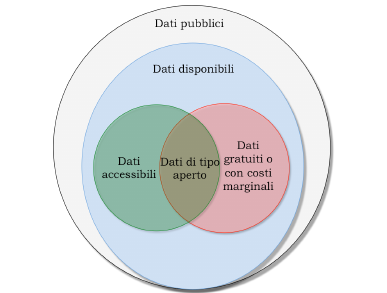
\includegraphics[width=250px]{od_classificazione.png} 
  \end{figure}
\end{frame}

\section{Licenze}

\begin{frame}
\frametitle{Licenze}
  Sempre nelle linee guida, l'AgID identifica il seguente schema per il \emph{licensing}
  degli Open Data
  \begin{figure}
    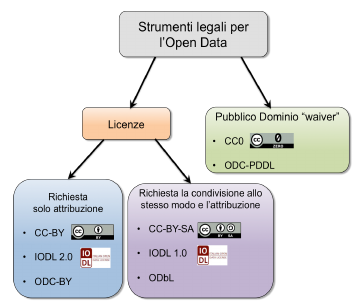
\includegraphics[width=180px]{licenze.png} 
  \end{figure}
\end{frame}

\begin{frame}
\frametitle{Licenze - Pubblico Dominio}
  Con le licenze \emph{waiver} l'autore rinuncia ad ogni diritto sull'opera. In tal modo
  l'opera diventa di \emph{pubblico dominio}. Citiamo il testo della licenza
  \emph{Creative Commons 0 (CC0)}\footnote{http://creativecommons.org/publicdomain/zero/1.0/}
  \vspace{\baselineskip}
  
   \begin{quote}
The person who associated a work with this deed has dedicated the work to the public domain by waiving all of his or her rights to the work worldwide under copyright law, including all related and neighboring rights, to the extent allowed by law.

You can copy, modify, distribute and perform the work, even for commercial purposes, all without asking permission.
   \end{quote}
   
   \uncover<2->{Nelle linee guida dell'AgID si rileva come l'utilizzo di licenze appartenenti a questa categoria sia inopportuno
per i dati delle pubbliche amministrazioni in quanto \emph{``prevede il rilascio dei diritti
morali che sono inalienabili, indisponibili, imprescrittibili secondo le norme nazionali ed europee. In
particolare poi tutti i beni del demanio culturale (art. 10 e art. 53, Codice dei beni culturali, D.lgs. 22
gennaio 2004, n. 42) per loro natura sono indisponibili e quindi è richiesta esplicitamente la menzione
di informazioni di attribuzione.''}}

\end{frame}

\begin{frame}
\frametitle{Licenze - Open Data}

Nell'ambito degli Open Data, alcune restrizioni che \`e possibile prevedere nella licenza
applicata ai dati sono:

\begin{itemize}[<+->]
 \item \emph{Attribution (BY)} dover attribuire in maniera opportuna la paternit\`a dei dati, 
 \item \emph{Share-Alike (SA)} distribuire eventuali lavori derivati con la stessa identica licenza che governa il lavoro originale;
\end{itemize}
\end{frame}

\begin{frame}
\frametitle{Licenze - Creative Commons Attribution}
La licenza \emph{Creative Commons - Attribution 3.0 (CC-BY 3.0)}\footnote{\url{http://creativecommons.org/licenses/by/3.0/it/deed.it}}
permette quindi di
\begin{itemize}
 \item \emph{Condividere} - riprodurre, distribuire, comunicare al pubblico, esporre in pubblico, 
 rappresentare, eseguire e recitare questo materiale con qualsiasi mezzo e formato;
 \item \emph{Modificare} — remixare, trasformare il materiale e basarti su di esso per le tue opere
per qualsiasi fine, anche commerciale.
\end{itemize}


\uncover<2->{
Le restrizioni imposte sono le seguenti:
  \begin{itemize}
   \item \emph{Attribuzione} - Devi riconoscere una menzione di paternità adeguata, fornire un link alla licenza e indicare se sono state effettuate delle modifiche. Puoi fare ciò in qualsiasi maniera ragionevole possibile, ma non con modalit\`a tali da suggerire che il licenziante avalli te o il tuo utilizzo del materiale;
   \item \emph{Divieto di restrizioni aggiuntive} - Non puoi applicare termini legali o misure tecnologiche che impongano ad altri soggetti dei vincoli giuridici su quanto la licenza consente loro di fare. 
  \end{itemize}

}
\end{frame}

\begin{frame}
\frametitle{Licenze - Creative Commons Attribution Share Alike}
La licenza \emph{Creative Commons - Attribution Share Alike 3.0 (CC-BY-SA 3.0)}\footnote{\url{http://creativecommons.org/licenses/by-sa/3.0/it/deed.it}}
permette quindi di
\begin{itemize}
 \item \emph{Condividere} - riprodurre, distribuire, comunicare al pubblico, esporre in pubblico, 
 rappresentare, eseguire e recitare questo materiale con qualsiasi mezzo e formato;
 \item \emph{Modificare} — remixare, trasformare il materiale e basarti su di esso per le tue opere
per qualsiasi fine, anche commerciale.
\end{itemize}


\uncover<2->{
Le restrizioni imposte sono le seguenti:
  \begin{itemize}
   \item \emph{Attribuzione} - Devi riconoscere una menzione di paternità adeguata, fornire un link alla licenza e indicare se sono state effettuate delle modifiche. Puoi fare ciò in qualsiasi maniera ragionevole possibile, ma non con modalit\`a tali da suggerire che il licenziante avalli te o il tuo utilizzo del materiale;
   \item \emph{Divieto di restrizioni aggiuntive} - Non puoi applicare termini legali o misure tecnologiche che impongano ad altri soggetti dei vincoli giuridici su quanto la licenza consente loro di fare; 
  \uncover<3->{
   \item \emph{Stessa Licenza} - Se remixi, trasformi il materiale o ti basi su di esso, devi distribuire i tuoi contributi con la stessa licenza del materiale originario.
  }
  \end{itemize}
}
\end{frame}

\begin{frame}
\frametitle{Licenze - Compatibilit\`a}
  La seguente matrice indica quali licenze possono essere applicate ad un'opera derivata
  in base alla licenza con cui \`e rilasciata l'opera originaria.\footnote{Una versione estesa di questa tabella \'e presente nelle
  linee guida nazionali per la valorizzazione del patrimonio informativo pubblico dell'AgID.} 
  \begin{figure}
    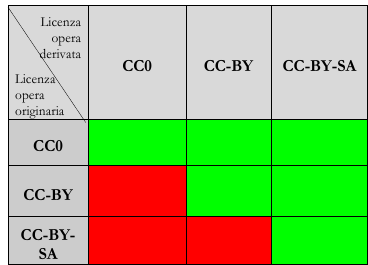
\includegraphics[width=180px]{compatibilita_licenze.png} 
  \end{figure}
\end{frame}

\section{Formati}
\begin{frame}
\frametitle{Formati Aperti - Open Definition}
La Open Definition fornisce indicazioni precise sul \emph{formato} nel quale vanno forniti i dati.
\vspace{\baselineskip}

\emph{1.3 Open Format}
\vspace{\baselineskip}

The work must be provided in a convenient and modifiable form such that there are no unnecessary 
technological obstacles to the performance of the licensed rights. Specifically, data should be machine-readable, 
available in bulk, and provided in an open format (i.e., \emph{a format with a freely available published specification 
which places no restrictions, monetary or otherwise, upon its use}) or, at the very least, 
can be processed with at least one free/libre/open-source software tool.
\vspace{\baselineskip}

\uncover<2->{
Nel \emph{Codice per l'Amministrazione Digitale} viene riportata la seguente definizione:
\vspace{\baselineskip}

\emph{formato dei dati di tipo aperto}: un formato di dati reso pubblico, documentato esaustivamente e neutro rispetto agli
strumenti tecnologici necessari per la fruizione dei dati stessi.
}
\end{frame}

\begin{frame}
\frametitle{Formati Aperti - Linee Guida AgID}

Nelle linee guida emanate dall'AgID viene fatta una distinzione tra \emph{dati} e
\emph{documenti}:

\begin{quote}
[...] \`e possibile convenire che il documento, in generale, rappresenta una
collezione di informazioni (e.g., dati, contenuti multimediali, atti e narrazione di eventi) pensato
principalmente per essere direttamente leggibile in forma scritta e visuale da parte di persone.
\end{quote}
\vspace{\baselineskip}

Vengono quindi indicati alcuni formati da utilizzare per la pubblicazione di dati e documenti
\end{frame}


\begin{frame}
\frametitle{Formati Aperti - Dati}
Alcuni formati aperti per i dati sono:
\vspace{\baselineskip}

\begin{itemize}[<+->]
 \item \emph{Comma Separated Values (CSV)} -  formato di file testuale usato per rappresentare
 dati in forma tabellare; Alcuni esempi sono disponibili in \url{http://opendata.comune.catania.gov.it}.
 
 \item \emph{eXtensible Markup Language (XML)}\footnote{\url{http://www.w3.org/TR/xml/}} linguaggio di marcatura, usato per la rappresentazione di dati strutturati.
 
 \item \emph{JavaScript Object Notation (JSON)}\footnote{\url{http://www.ietf.org/rfc/rfc4627.txt}, \url{http://json.org}} - formato per dati \emph{strutturati}, analogo a XML
 ma pi\`u \emph{leggero}. Facilmente trattabile con JavaScript.
 
 \item \emph{Resource Description Framework (RDF)}\footnote{\url{http://www.w3.org/RDF/}} linguaggio sviluppato nell'ambito dei sistemi di rappresentazione
 della conoscenza. Il modello dati \`e basato sui \emph{grafi}. Permette il collegamento tra dati. Ammette diverse \emph{serializzazioni}: RDF/XML, N3, turtle, JSON-LD.
 
 \item \emph{Web Ontology Language (OWL)}\footnote{\url{http://www.w3.org/OWL/}} basato su RDF, ammette una \emph{semantica formale}
 derivata dalle logiche descrittive.
\end{itemize}
\end{frame}

\begin{frame}
\frametitle{Formati Aperti - Dati Geografici}
Per i dati geografici vengono indicati alcuni formati specifici:
\vspace{\baselineskip}
\begin{itemize}[<+->]
    \item \emph{Shapefile\footnote{\url{http://www.esri.com/library/whitepapers/pdfs/shapefile.pdf,}}} - standard de-facto per la rappresentazione dei dati dei sistemi informativi
    geografici (GIS). I dati sono di tipo vettoriale. Creato da ESRI.
    \item \emph{KML\footnote{\url{ http://www.opengeospatial.org/standards/kml}}} - formato basato su XML per rappresentare dati geografici. Nato con Google, \`e
    diventato poi uno standard OGC.
    \item \emph{GeoJSON\footnote{\url{http://geojson.org/}}} - formato per la rappresentazione e l'interscambio dei dati territoriali in
    forma vettoriale, basato su JSON.
    \item \emph{Geography Markup Language (GML)\footnote{\url{http://www.opengeospatial.org/standards/gml}}} - formato di scambio per i dati territoriali basato su XML. 
    Standard ISO 19136:2008.
    \item \emph{GeoPackage\footnote{\url{http://www.geopackage.org}}} - formato aperto per la rappresentazione di dati geografici alternativo al formato 
    shapefile. Esso supporta SpatiaLite, estensione di SQLite. Lo standard \`e riconosciuto dall'Open
    Geospatial Consortium (OGC).
\end{itemize}
\end{frame}

\begin{frame}
\frametitle{Formati Aperti - Documenti}
Riportiamo alcuni formati aperti per i documenti (atti, delibere, certificazioni, \ldots):
\vspace{\baselineskip}

\begin{itemize}[<+->]
  \item \emph{Open Document Text (ODT)} - standard per documenti testuali basato su XML. Mantenuto da OASIS.
  \item \emph{Open Document Spreadsheet (ODS)} - standard per fogli di calcolo basato su XML. Mantenuto da OASIS.
  \item \emph{Open Document Presentation (ODP)} - standard per documenti di presentazione basato su XML. Mantenuto da OASIS.
  \item \emph{Portable Document Format (PDF)} - formato per la rappresentazione di documenti contenenti testo e immagini 
    indipendente dalla piattaforma (ISO/IEC 32000-1:2008). Creato da Adobe.
  \item \emph{Akoma Ntoso}\footnote{\url{http://www.akomantoso.org/}} - linguaggio basato su XML per la rappresentazione di documenti giuridici.
    Attualmente in fase di approvazione presso il consorzio OASIS. Utilizzato dal Parlamento
    Europeo e dalla Commissione Europea per i documenti legislativi.
\end{itemize}
\end{frame}

\section{Metadati}

\begin{frame}
  \frametitle{Metadati}
  L'aggiunta di \emph{metadati} associati ai daset o ai dati garantisce una maggiore
  \emph{raggiunggibilit\'a} dei dati di interesse da parte degli utenti. Ad esempio
  favorisce l'indicizzazione da parte de motori di ricerca.
  \vspace{\baselineskip}
  
\uncover<2->{
  Questa pratica pu\`o avere anche altre importanti funzioni:
  \begin{itemize}[<+->]
   \item \emph{titolarit\`a} - chi ha prodotto il dato e chi lo mantiene;
   \item \emph{tempestivit\`a} - quale \`e la frequenza di aggiornamento dei dati, se il dato pu\`o essere
   considerato ancora attendibile e per quanto tempo ancora;
   \item \emph{provenienza} - come \`e stato formato il dato ed eventualmente dalla combinazione ed elaborazione
   di quali dataset \emph{primari} \`e stato derivato o importato. 
  \end{itemize}
} 

\uncover<2->{
  Nelle Linee Guida AgID vengono presentate alcune tipologie di metadati \emph{obbligatori} e
  altre di metadati \emph{consigliati}. I metadati obbligatori si suddividono a loro volta in 
  metadati \emph{universalmente} obbligatori, che devono essere 
  sempre presenti, e metadati che sono richiesti solo al in presenza di particolari condizioni.
  \vspace{\baselineskip}
}  

\end{frame}

\begin{frame}
  \frametitle{Metadati Universalmente Obbligatori}

  Riportiamo i metadati sempre obbligatori.
  
  \begin{figure}
    \begin{itemize}[<+->]
      \item \tt{publisher} - soggetto che pubblica il dataset. Spesso coincide con \tt{creator}.
      \item \tt{creator} - soggetto che ha prodotto il dataset.
      \item \tt{rightsHolder} - indica il soggetto o l’organizzazione che detiene e gestisce i diritti sul dataset.
      \item \tt{title} - il titolo del dataset.
      \item \tt{description} - una descrizione in linguaggio naturale del dataset.
      \item \tt{modified} - la data di ultimo aggiornamento.
      \item \tt{accrualPeriodicity} - frequenza di aggiornamento dei dati.
      \item \tt{license} - indica la licenza utilizzata.
      \item \tt{keyword} - parole chiave, separate da virgole, che descrivono il dataset.
    \end{itemize}
    \caption{Metadati Obbligatori}
  \end{figure}
\end{frame}

\begin{frame}
  \frametitle{Metadati Condizionatamente Obbligatori}

  Riportiamo i metadati sempre obbligatori solo in particolari condizioni.
  
  \begin{figure}
    \begin{itemize}[<+->]
    \item \tt{identifier} - solo in caso di LOD, URI che identifica il dataset universalmente.
    \item \tt{spatial} - se i dati hanno significato solo all'interno di una determinata copertura spaziale. 
    \item \tt{temporal} - se i dati hanno significato solo all'interno di una determinata copertura temporale.
    \item \tt{language} - la lingua con cui sono espressi i dati (vedi anche RFC 4646). Obbligatorio solo se 
      la comprensione dei dati richiede laconoscenza di una determinata lingua.
    \item \tt{byteSize} - la dimensione del dataset. Richiesto se la dimensione del dataset supera i 200 MB.
    \item \tt{accessURL} - se il dataset ha un endpoint di accesso  a cui possiamo
    sottoporre le query sul dataset, indica l'indirizzo di questo.
    \item \tt{downloadURL} - se il dataset risiede in un file scaricabile, indica la posizione fisica del file.
    \end{itemize}
    \caption{Metadati Condizionatamente Obbligatori}
  \end{figure}
\end{frame}
\end{document}

\begin{frame}
  \frametitle{Metadati Condizionatamente Obbligatori}
  
  I metadati sono solitamente associati ai dataseti. Esistono schemi di metadatazione che permettono
  di associare informazioni
  \begin{itemize}
   \item a cataloghi di dataset (DCAT) o
   \item a singoli dati all'interno del dataset (PROV).
  \end{itemize}
\end{frame}